%!TEX root = draft.tex
\section{Parallel algorithms}\label{sec:parallel algorithms}
\subsection{Grid management}
Adaptive tree-based grids can significantly reduce the computational cost of level-set methods by restricting the fine grid close to the interface where it is most needed \cite{Strain:99:Tree-Methods-for-Mov}. Moreover, adaptive tree-based grids are easy to generate in the presence of a signed-distance level-set function \cite{Min;Gibou:07:A-second-order-accur} and can efficiently be encoded using a tree datastructure \cite{Samet:90:Applications-of-Spat}. To develope scalable parallel algorithms on these grids, it is necessary to parallelize the datastructure and grid manipulations method such as refinement and coarsening of cells as well as provide with a fast method for grid partitioning and load balancing. \texttt{p4est} library \cite{p4est-github} is a collection of such parallel algorithms that has recently emerged and shown to scale up to 200,000 processors \cite{Burstedde;Wilcox;Ghattas:11:p4est:-Scalable-Algo}.

In \texttt{p4est} the adaptive grid is represented as a non-overlapping collection of trees that are rooted in individual cells of a common coarse grid (c.f. figure \ref{fig:p4est_zcurve}). This common coarse grid, which we will refer to as the ``macromesh'', can in general be an unstructured quadrilateral, in two spatial dimensions, or hexahedral mesh, in three spatial dimensions. In this article, however, we shall limit ourselves to simple uniform Cartesian macromeshes. Moreover it is implicitly assumed that the macromesh is small enough that can be entirely replicated on all processors. For instance, in many of the applications that we are interested in this paper the macromesh simply a single cell. \texttt{p4est} allows for arbitrary refinement and coarsening criteria through defining callback functions. In this article the refinement criteria is chosen based on the distance of individual cells to the interface. Specifically a cell $C$ is marked for refinement if:
\be
\min_{\forall v \in V(C)} |\phi| \le \frac{L D}{2}.
\label{eq:refine}
\ee
Conversely an existing cell is marked for coarsening if:
\be
\min_{\forall v \in V(C)} |\phi| > L D.
\label{eq:coarsen}
\ee
Here $V(C)$ denotes the set of all vertices of cell $C$, $L$ denotes the Lipschitz constant of the level-set function, and $D$ denotes the diagonal size of cell $C$. We refer to section 3.2 of \cite{Burstedde;Wilcox;Ghattas:11:p4est:-Scalable-Algo} for details on parallel refinement and coarsening algorithms used in \texttt{p4est}.

Once the gird is adapted to the interface, it must be partitioned to ensure load balancing across processors. This is achieve by constructing a Z-curve that traverses the leaves of all trees in order of tree index (c.f. figure \ref{fig:p4est_zcurve}). A Z-curve is a Space Filling Curve (SFC) with the important property that cells with close Z-indecies are also geometrically close in the physical domain. This is beneficial since it both leads to reduction in MPI communication and improves the cache performance of several algorithms such as interpolation and finite difference calculations. For more details on parallel partitioning in \texttt{p4est} one may refer to section 3.3 of \cite{Burstedde;Wilcox;Ghattas:11:p4est:-Scalable-Algo}.
\begin{figure}[hbtp]
\begin{center}
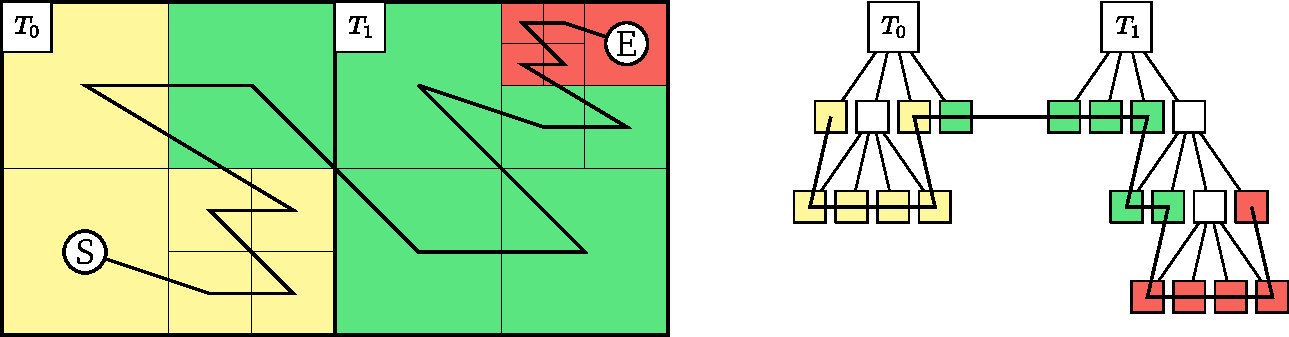
\includegraphics[width = \columnwidth]{figures/p4est_zcurve.pdf}
\caption{Left: A ``forest'' made up of two trees $k_0$ and $k_1$. Parallel partitioning is achieved by first constructing a Z-curve which starts at cell ``S'' and ends at cell ``E''. Next this tree is split up among processors either uniformly or by assigning different weights to cells. Here processors are represented via different colors. Note how use of Z-curve naturally leads to clustering of most cells in each processor domain. Right: Schematic of a tree data structure representing the forest and its partitioning.}
\label{fig:p4est_zcurve}
\end{center}
\end{figure}
Aside from grid manipulation and partitioning, we use two additional features of \texttt{p4est}, namely generation of ghost layer cells and creating a globally unique node indexing. These algorithms are detailed in sections 3.5 and 3.6 of \cite{Burstedde;Wilcox;Ghattas:11:p4est:-Scalable-Algo}. An important feature of our algorithms is that they are designed for non-graded trees. This is important because we can entirely skip tree balancing which was shown to be one of most time consuming parts of grid adaptation in \texttt{p4est} \cite{Burstedde;Wilcox;Ghattas:11:p4est:-Scalable-Algo}.

Finally, in \texttt{p4est} trees are linearized, i.e. only the leaves are explicitly stored. However, all of algorithms considered here require explicit knowledge of the entire tree. As a result we introduce a simple algorithm, called \texttt{Reconstruct}, which recreates a local representation of the entire ``forest'' that is only adapted to local cells and, potentially, the ghost layer. This approach is similar to the ideas introduced in \cite{Bangerth;Burstedde;Heister;etal:11:Algorithms-and-data-} and our tests show that in a typical application they usually amount to less that $1\%$ of the entire runtime. Algorithm \ref{alg:reconstruction} illustrates how this reconstruction is performed. Given a forest and a layer of ghost cells from \texttt{p4est}, the algorithm generates a local representation of forest by recursively refining from the root until reaching the same level and location of all leaves in \texttt{p4est} and \texttt{ghost}. Note that algorithm \ref{alg:reconstruction} does not involve any communication and is load balanced. Figure \ref{fig:reconstruction} illustrates an application of algorithm \ref{alg:reconstruction}. Note how each processor has independently generated a local representation of the forest that is refined to match the same leaves as in the global forest and ghost layer.
% , and has an average runtime complexity of $\mathcal{O}\left((n_l + n_g)\log_{2^d}N\right)$ for well-balanced trees in $d$ dimensions. Here, $n_l$ and $n_g$ are the number of local and ghost cells, respectively, and $N$ is the global number of cells.
\begin{algorithm}[htbp]
\caption{$H \gets \texttt{Reconstruct (}G\texttt{)}$}\label{euclid}
\begin{algorithmic}[1]
\State $H \gets G.\texttt{macromesh()}$
\For {$tr : G.\texttt{local\_trees()}$} \Comment{traverse local cells}
	\For {$q : tr.\texttt{cells()}$}
		\State $H.\texttt{update\_tree(} tr, q \texttt{)}$
	\EndFor
\EndFor

\For {$q : G.\texttt{ghost\_cells()}$} \Comment{traverse ghost cells}
	\State $H.\texttt{update\_tree(} q.\texttt{tree()}, q \texttt{)}$
\EndFor

\State \Return $H$
\\
\Function{$H.\texttt{update\_tree}$}{$tr, q$}   \Comment{recursive reconstruction}
	\State $q_l \gets H.\texttt{root(}tr\texttt{)}$
	\While{$q_l.\texttt{level()} \not= q.\texttt{level()} $}
		\If {$q_l.$\texttt{is\_leaf()}} $q_l$\texttt{.split()}
		\EndIf
		\State $h \gets q_l.\texttt{length()} / 2$ \Comment{select the next child based on direction}
		\State $i \gets q.x \ge q_l.x + h$
		\State $j \gets q.y \ge q_l.y + h$
		\State $k \gets q.z \ge q_l.z + h$

		\State $q_l \gets q_l.\texttt{child(} i, j, k \texttt{)}$
	\EndWhile	
\EndFunction
\end{algorithmic}
\label{alg:reconstruction}
\end{algorithm}

\begin{figure}[htbp]
\begin{center}
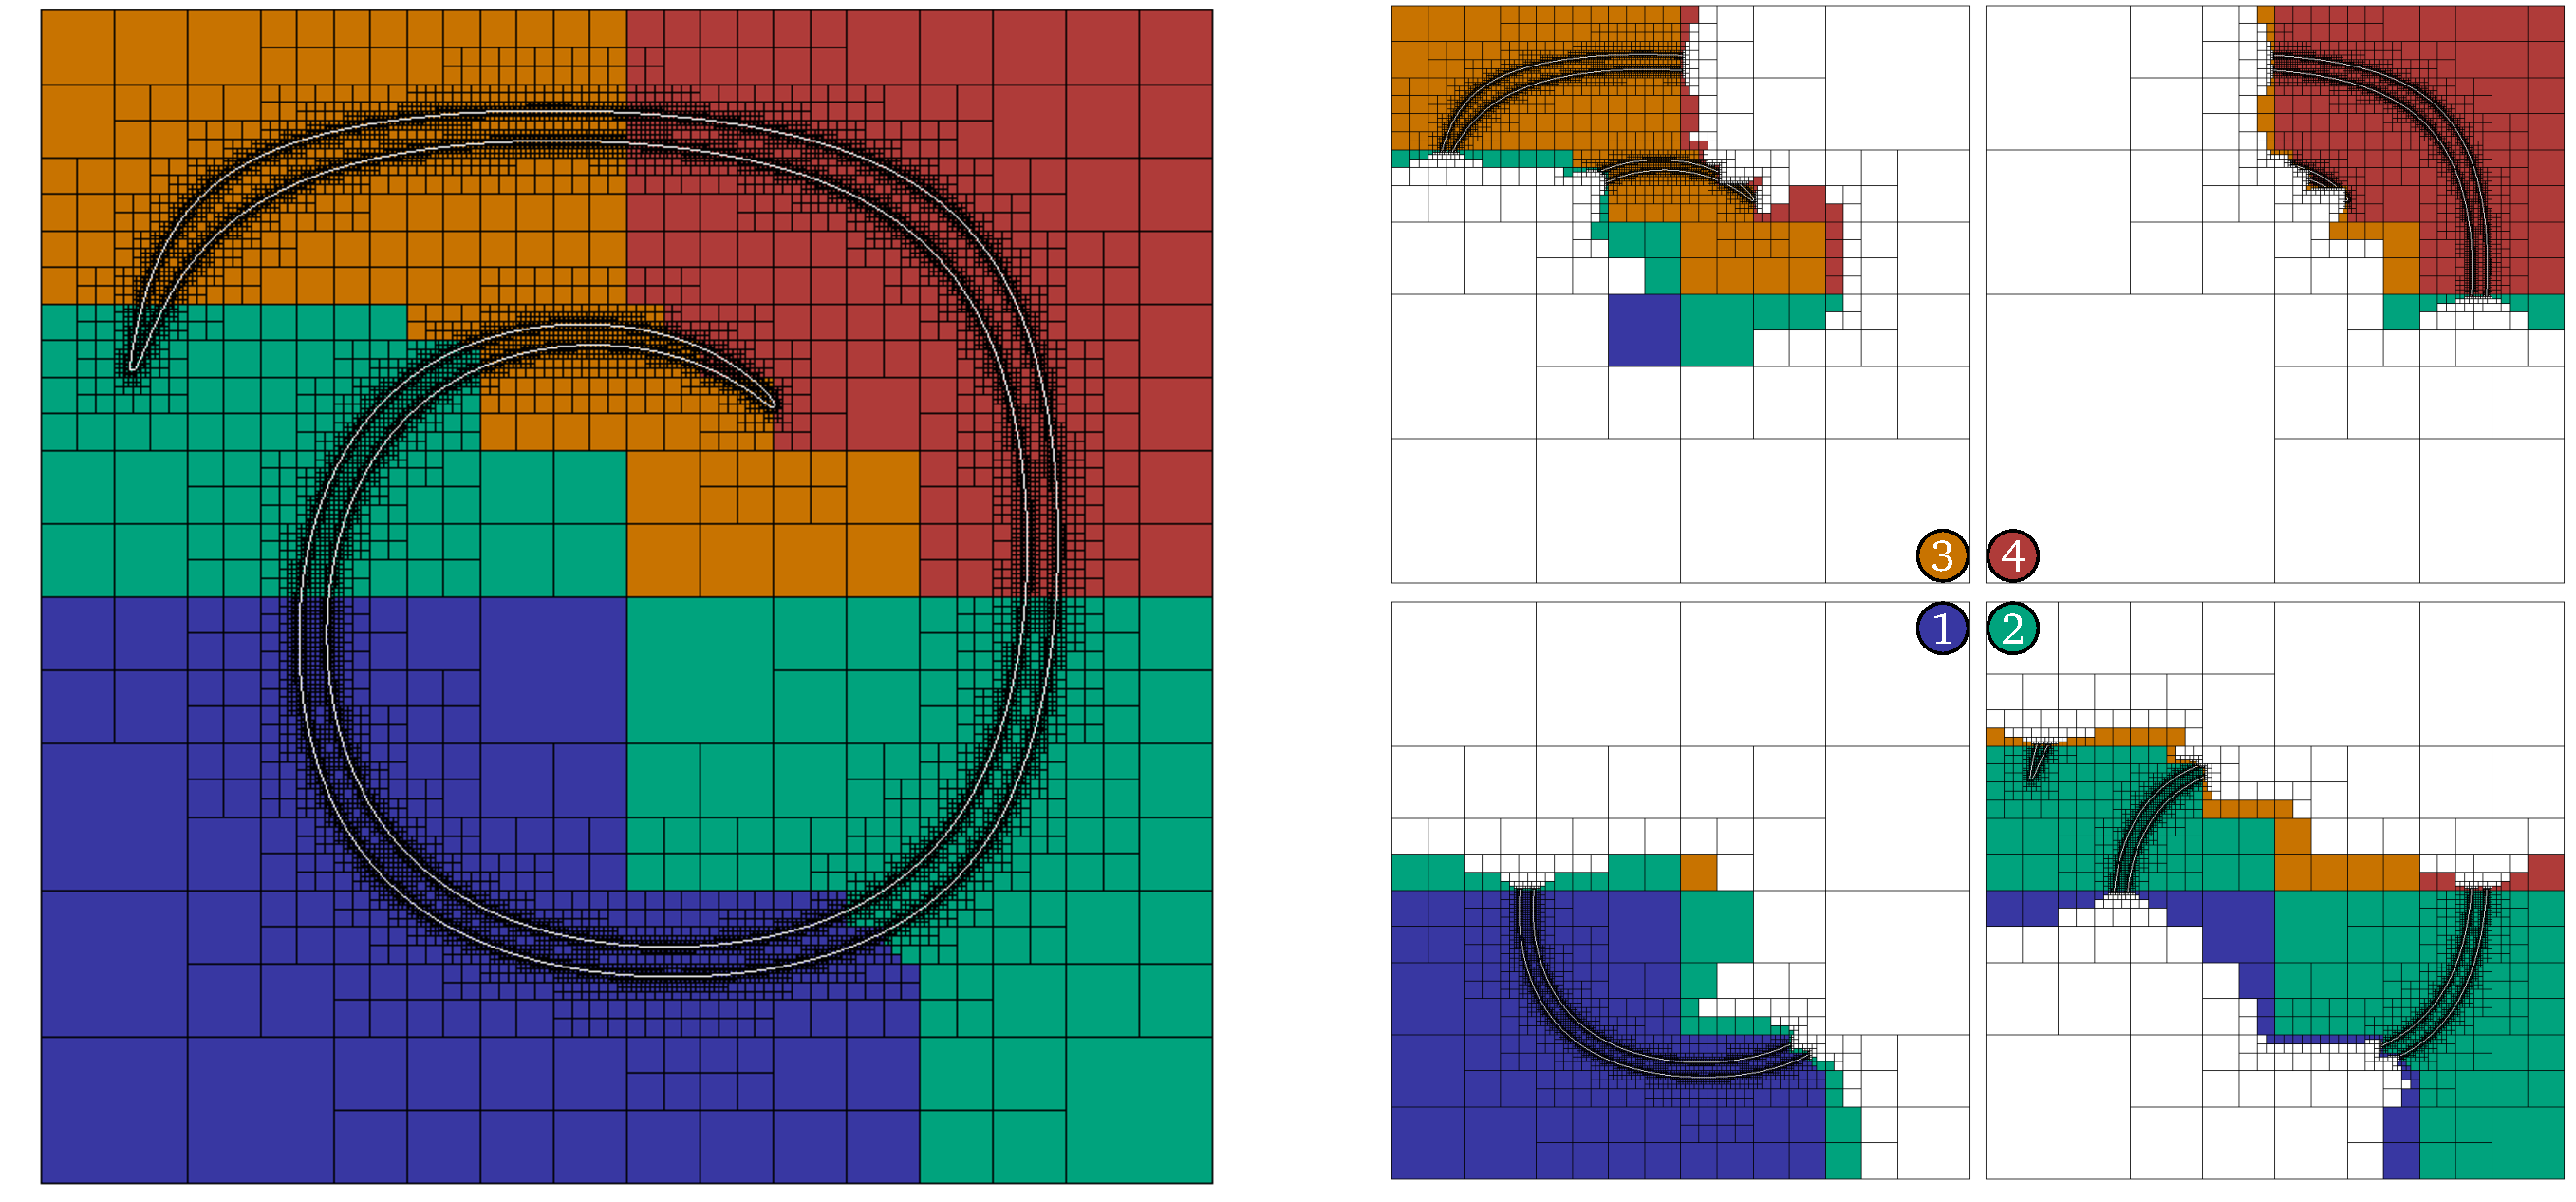
\includegraphics[width = \textwidth]{figures/reconstruct.pdf}
\end{center}
\caption{Left: A forest refined close to an interface and partitioned among four processors as indicated by colors. Right: Each processor independently recreates a local forest which is refined to match the global grid and is as coarse as possible elsewhere. Note that empty cells are fictitious, i.e. they are only required to generate the hierarchal structure and are not matched by any corresponding cell in the global forest.}
\label{fig:reconstruction}
\end{figure}

\subsection{Semi-Lagrangian method}
As indicated earlier, we use the Semi-Lagrangian method to solve equation \eqref{eq:ls} when the velocity field is externally generated, i.e. does not depend on level-set function itself. Let us rewrite equation \eqref{eq:ls} along the characteristic curve $\mathbf{X}(t)$ as:
\be
\left\{
\begin{array}{rcl}
\dfrac{\text{d} \mathbf{X}}{\text{d} t} &=& \mathbf{V}, \\ [3ex]
\dfrac{\text{d} \phi(\mathbf{X}(t), t)}{\text{d} t} &=& 0.
\end{array}
\right.
\label{eq:sl}
\ee
The Semi-Lagrangian method integrates equations \eqref{eq:sl} backward in time, i.e. starting from the grid $G^{n+1}$ \footnote{$G^{n+1}$ itself is computed in an iterative fashion as explained later on.}, we simply write $\phi^{n+1}(\mathbf{X}^{n+1}) = \phi(\mathbf{X}(t^{n+1}), t^{n+1}) = \phi(\mathbf{X}(t^n), t^n) = \phi^n(\mathbf{X}_d)$. Here the characteristic curves are chosen such that $\mathbf{X}(t^{n+1})$ are simply the coordinates of grids points of $G^{n+1}$. Moreover $\mathbf{X}_d$ are the departure points which are computed using the second-order midpoint method \cite{Min;Gibou:07:A-second-order-accur}:
\bea
\mathbf{X}^\star &=& \mathbf{X}^{n+1} - \frac{\Delta t}{2} \mathbf{V}^{n}(\mathbf{X}^n),	   \label{eq:xstar}      \\
\mathbf{X}_d     &=& \mathbf{X}^{n+1} - \Delta t \mathbf{V}^{n+\frac{1}{2}}(\mathbf{X}^\star), \label{eq:xdeparture}
\eea
where $\mathbf{V}^{n+\frac{1}{2}}$ is obtained via extrapolation from previous times, i.e.:
\be
\mathbf{V}^{n+\frac{1}{2}} = \frac{3}{2} \mathbf{V}^n - \frac{1}{2}\mathbf{V}^{n-1}. \label{eq:vn_p_half}
\ee

Note that all values at the intermediate point, $\mathbf{X}^\star$, and departure point, $\mathbf{X}_d$, must be calculated via interpolation from previous grids, $G^{n}$ and $G^{n-1}$. Here we use the stabilized second-order interpolation for $\phi(\mathbf{X}_d)$ and the multi-linear interpolation for $\mathbf{V}^{n+\frac{1}{2}}(\mathbf{X}^\star)$ \cite{Min;Gibou:07:A-second-order-accur}. Although parallelization of the interpolation process on a shared-memory machine is trivial, the same cannot be said for distributed-memory machines. In fact, the parallel interpolation algorithm \ref{alg:interpolation} is probably the most important contribution of this article. Complication arises because not all calculated departure points will reside in the domain of current processor. Moreover, due to the irregular shape of partitions, we cannot be certain that they are entirely owned by neighboring processors. At best we can only expect that their location are bounded by a halo of width $w \le \text{CFL} \: \Delta x_{\min}$ around the local partition. Of course if one enforces $\text{CFL} \le 1$, one can ensure that the halo is bounded by the ghost layer which significantly simplifies the communication problem. This assumption, however, defeats the purpose of using Semi-Lagrangian in the first place since we are interested in large values of $\text{CFL}$ number.

One remedy to this problem, proposed in \cite{Thomas;Cote:95:Massively-parallel-s} for uniform grids, is to increase the size of ghost layer to $\lceil \text{CFL} \rceil$. For large values of $\text{CFL}$ number, however, this approach can substantially increase the communication volume. Moreover, this simple approach does not work in the process of generating $G^{n+1}$ due to repartitioning. An alternative approach would be to handle local and remote interpolations separately. Our remote interpolation algorithm is composed of three separate phases. In the first phase, which we call buffering, every processor searches for all departure points inside the local tree. If the point is owned by a local cell, it is added to a local buffer, otherwise we find the processor which owns the point and add the point to a separate buffer belonging to the found rank. Note that searching the point in the local tree is performed recursively, similar to the \texttt{UpdateLocalTree} function in algorithm \ref{alg:reconstruction}. The owner's rank is found by computing the Z-index of the point and then using binary search on the Z-curve. This is already implemented in \texttt{p4est} and explained in details in section 2.5 of \cite{Burstedde;Wilcox;Ghattas:11:p4est:-Scalable-Algo}.

Once buffering is done, every processor knows exactly how many messages it needs to send and to which processors. This also implicitly defines processors that will later on send a reply message to this processor. However, at this point no one knows which processors they should expect a message from. We solve this problem using a simple \textit{communication matrix} (see figure \ref{fig:communication}). Other approaches for solving this problem could include using non-blocking collective or one-sided communication operations introduced in the MPI-3 standard \cite{MPI_ref, sparse dynamic exchange protocol paper}. Although these algorithms have better theoretical communication complexities, we did not see any difference in the runtime or scalability of algorithm \ref{alg:interpolation} when using them. 

\begin{figure}[htbp]
\begin{center}
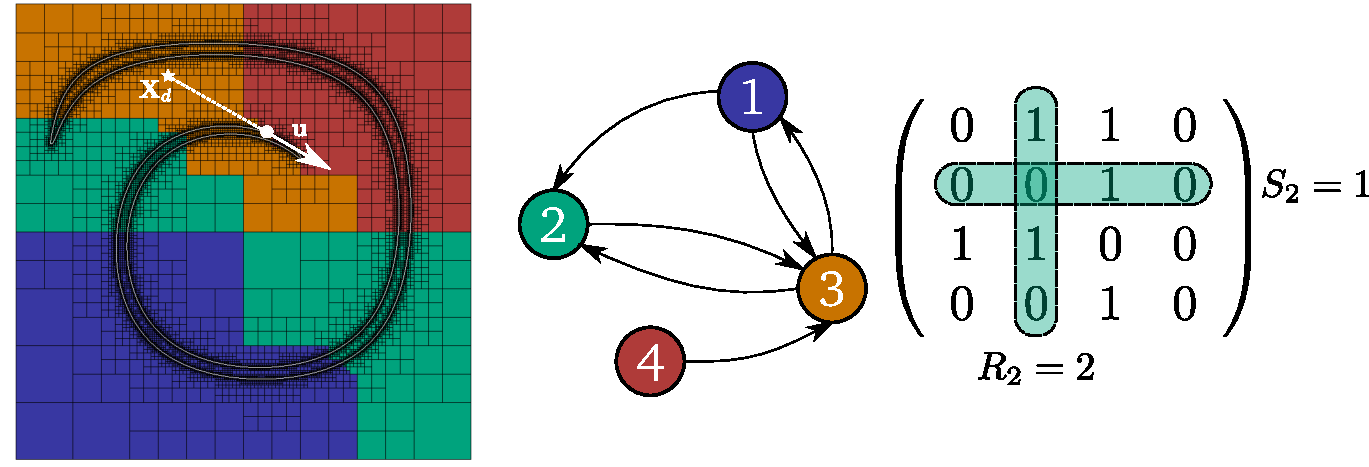
\includegraphics[width = \textwidth] {figures/communication.pdf}
\end{center}
\caption{Left: Location of back-traced points depends on the magnitude of local velocity and time-step. Although departure distance is bounded by $\text{CFL} \: \Delta x_{\min}$, one cannot make any special assumption about receiving rank without explicit searching of the entire Z-curve. Moreover, the receiving processor has no prior knowledge about which processors to check for incoming messages nor does it know anything about the possible message length (i.e. number of points). Middle: A directed graph illustrating the communication pattern among processors with arrows representing the direction that messages are sent. Right: The adjacency matrix of communication graph. For each row, sum of all columns represents the number of sent messages. Conversely, for each column, sum of all rows represents number of messages that need to be received. As detailed in algorithm \ref{alg:interpolation} this information is enough to build a parallel interpolation scheme.}
\label{fig:communication}
\end{figure}

To solve the communication problem, we first compute the adjacency matrix of the communication pattern, i.e. we construct the matrix $A_{P \times P}$ such that:
\ben
a_{ij} = 
\left\{
\begin{array}{lr}
1 \hspace{5 mm} \text{if processor `\textit{i}' sends a message to processor `\textit{j}',} \\
0 \hspace{5 mm} \text{otherwise.}
\end{array}
\right.
\een
Note that this matrix is also distributed among processors, i.e. each row is owned by a separate rank. Next, we compute:
\ben
S_i = \sum_j a_{ij} \hspace{5 mm} \text {and} \hspace{5 mm} R_i = \sum_j a_{ji}
\een
where $S_i$ and $R_i$ denote the number of sent and received messages respectively. While $S_i$ can be computed trivially, a reduction operation is required for computing $R_i$. For instance, this can be achieved using a single \texttt{MPI\_Reduce\_scatter} function call. The last phase of interpolation involves overlapping the computation of interpolated values for local points with the communication of data between processors. This is done by alternating between local calculations and probing for incoming messages from other processors. Interpolation is finished once values for all local points have been calculated and all remote requests have been processed (see algorithm \ref{alg:interpolation}).
\begin{algorithm}[htbp]
\caption{$values \gets \texttt{Interpolate (}H, \mathbf{X}\texttt{)}$}\label{euclid}
\begin{algorithmic}[1]
\State $col \gets 0, buff \gets null$ \Comment{Phase I -- buffering}
\For {$\mathbf{p} : \mathbf{X}$} 
	\State $[r, cell] \gets H.\texttt{search(}\mathbf{p}\texttt{)}$ \Comment{search for the owner's rank and cell}
	\If {$r = mpirank$}
		\State $buff[r].\texttt{push\_back(}\mathbf{p}, cell\texttt{)}$
	\Else
		\State $buff[r].\texttt{push\_back(}\mathbf{p}\texttt{)}$
		\State $col[r] \gets 1$
	\EndIf
\EndFor
\For {$r: mpisize$} \Comment{Phase II -- initiate communication and compute number of messages}
	\If {$col[r]$}
		\State $\texttt{MP\_Isend(}r, buff[r]\texttt{)}$
	\EndIf
\EndFor
\State  $S \gets \texttt{sum(}col\texttt{)}$ 
\State  $R \gets \texttt{MPI\_Reduce\_scatter(}col,\texttt{MPI\_SUM)}$
\State $done \gets false, it \gets buff[mpirank].\texttt{begin()}$
\While {$!done$} \Comment{Phase III -- main loop}
	\If {$it \not= buff[mpirank].\texttt{end()}$}
		\State $values \gets \texttt{process\_local(}it\texttt{)}$ \Comment{process local interpolations}
		\State $\texttt{++}it$
	\EndIf
	\If {$R > 0$} \Comment{process queries sent from remote processors}
		\State $[msg, st] \gets \texttt{MPI\_Iprobe()}$
		\If {$msg$}
			% \State $values \gets \texttt{MPI\_Recv(}st.\texttt{MPI\_SOURCE)}$ \Comment{}
			\State $val\_buff \gets \texttt{process\_queries(}st\texttt{)}$ \Comment{receive, search, and interpolate values}
			\State $\texttt{MPI\_Isend(}st.\texttt{MPI\_SOURCE},val\_buff\texttt{)}$ \Comment{send back interpolated values}
			\State $R\texttt{--}$
		\EndIf
	\EndIf
	\If {$S > 0$} \Comment{process replies sent to our queries}
		\State $[msg, st] \gets \texttt{MPI\_Iprobe()}$
		\If {$msg$}
			\State $values \gets \texttt{process\_replies(}st.\texttt{MPI\_SOURCE)}$ \Comment{receive remotely interpolated values}
			\State $S\texttt{--}$
		\EndIf
	\EndIf
	\State $done \gets S = 0 \: \And \: R = 0 \: \And \: it = buff[mpirank].\texttt{end()}$
\EndWhile
\State \Return $values$
\end{algorithmic}
\label{alg:interpolation}
\end{algorithm}

Using the interpolation algorithm \ref{alg:interpolation}, we close this section by presenting the final Semi-Lagrangian algorithm \ref{alg:semi-lagrangian}. The basic idea here is to start from an initial guess $G^{n+1}_0$ and modify the grid using refinement and coarsening criteria in \eqref{eq:refine} and \eqref{eq:coarsen} until convergence is obtained. Various options are available for $G^{n+1}_0$. For instance it is possible to start from the macromesh and only perform refinement steps until convergence. This choice, however, is not suitable since first few iterations do not contain many cells and there is little work for parallelism. Here we simply take the previous grid as the starting point, i.e. $G^{n+1}_0 = G^n$. Note that this iterative process is essentially unavoidable since the grid is based on the value of the level-set function at $t^{n+1}$, which itself is unknown and is to be defined on $G^{n+1}$. Nonetheless the process converges to the final grid in at most $l_{\max}$ steps where $l_{\max}$ denotes the maximum final depth of trees across all processors.
\begin{algorithm}[htbp]
\caption{$[G^{n+1}, \phi^{n+1}] \gets \texttt{SemiLagrangian (}G^n, \phi^n, \mathbf{V}^n, \mathbf{V}^{n-1}, \text{CFL}\texttt{)}$}\label{euclid}
\begin{algorithmic}[1]
\State $\Delta t_l \gets \text{CFL} \times \max \{\mathbf{V}^n\} / G^n.\texttt{hmin()}$
\State $\Delta t   \gets \texttt{MPI\_Allreduce(}\Delta t_l,\texttt{MPI\_MIN)}$
\State $H^n \gets \texttt{Reconstruct(} G^n\texttt{)}$ 
\State $G^{n+1}_0 \gets G^n$
\While {$true$}
	\State $\mathbf{X}_d  \gets \texttt{ComputeDeparturePoints(}G^{n+1}_0, \mathbf{V}^n, \mathbf{V}^{n-1}, \Delta t\texttt{)}$ \Comment{using equations \ref{eq:xstar} -- \ref{eq:vn_p_half}}
	\State $\phi^{n+1} \gets \texttt{Interpolate(}H^n, \textbf{X}_d\texttt{)}$
	\State $G^{n+1} \gets G^{n+1}_0.\texttt{refine\_and\_coarsen(}\phi^{n+1}\texttt{)}$ \Comment{using equations \ref{eq:refine} and \ref{eq:coarsen} as criteria}
	\If {$G^{n+1} \not= G^{n+1}_0$}
		\State $G^{n+1}.\texttt{partition()}$
		\State $G^{n+1}_0 \gets G^{n+1}$
	\Else
		\State \textbf{break}
	\EndIf
\EndWhile

\State \Return $[G^{n+1}, \phi^{n+1}]$
\end{algorithmic}
\label{alg:semi-lagrangian}
\end{algorithm}

\subsection{Reinitialization}
Successive application of algorithm \ref{alg:semi-lagrangian}, especially for large values of CFL number, potentially lead degrades the signed distance property of level-set function. It is thus important to reinitialize the level-set every few iterations, especially because the quality of generated grid heavily depends on the signed distance property. To achieve this property we solve the pseudo-time transient equation \eqref{eq:reinitialization} using the discretization scheme detailed in \cite{Min;Gibou:07:A-second-order-accur}. For completeness, we briefly review the scheme here. First equation \eqref{eq:reinitialization} is written in the following semi-discrete form:
\be
\frac{\text{d} \phi}{\text{d} \tau} + S(\phi_0) \left(\mathcal{H}_G(D^+_i \phi, D^-_i \phi) - 1 \right) = 0,
\label{eq:semidiscrete_reinit}
\ee
where $D^+_i \phi$ and $D^-_i \phi$ are the forward and backward derivatives in the $x_i$ direction and $\mathcal{H}_G$ is the Godunov Hamiltonian defined as:\
\ben
\mathcal{H}_G(a_i, b_i) = 
\left\{
\begin{array}{lcr}
	\sqrt{\sum_i \max\left(|a^+_i|^2, |b^-_i|^2\right)} & \hspace {5 mm} \text{if} & S(\phi_0) \le 0 \\
	\\
	\sqrt{\sum_i \max\left(|a^-_i|^2, |b^+_i|^2\right)} & \hspace {5 mm} \text{if} & S(\phi_0)  >  0 
\end{array}
\right.
,
\een
where $a^+ = \max(a, 0)$ and $a^- = \min(a, 0)$. Similar to \cite{Min;Gibou:07:A-second-order-accur}, equation \eqref{eq:semidiscrete_reinit} is integrated in time using the TVD-RK2 scheme using adaptive time-stepping to accelerate convergence to steady state. Since all computation is grid based, parallel implementation of this scheme is mostly trivial. However, one minor point requires further explanation. As suggested in \cite{Min;Gibou:07:A-second-order-accur}, one-sided derivatives $D^+_i \phi$ and $D^-_i \phi$ are computed using second order discretizations which require computation of second derivatives. To enable overlap between computation and communications when computing second derivatives and also integrating \eqref{eq:semidiscrete_reinit}, we use the following common technique. First, we label all local points, $L_p$, as either private, $P_p$, or boundary, $B_p$. Here, boundary points are the collection of all local points that are regarded as ghost point, $G_p$, on all other processors, i.e. $B_p = \underset{r,\;r\neq p}{\bigcup} G_r$. Private points are fined as the collection of all local points that are not a boundary point, i.e. $L_p = P_p\cup B_p$. Algorithm \ref{alg:overlap} illustrates how this labeling can help with computation/computation overlap of an arbitrary local operation $\phi^{n+1} \gets \mathcal{F}(\phi^n)$. Note that \texttt{p4est} library already includes all the primitives required for labeling local points without any further communication.

\begin{algorithm}[htbp]
\caption{$\phi^{n+1} \gets \texttt{Overlap (}\phi^n, \mathcal{F}\texttt{)}$}\label{euclid}
\begin{algorithmic}[1]
\For {$i:B_p$} \Comment{I -- perform computation on boundary points}
	\State $\phi^{n+1}_i \gets \mathcal{F}(\phi_i^n)$
\EndFor
\State $send\_req \gets \texttt{MPI\_Isend(}\phi^{n+1}_B\texttt{)}$ \Comment{II -- begin updating ghost values}
\State $recv\_req \gets \texttt{MPI\_Irecv(}\phi^{n+1}_G\texttt{)}$
\For {$i:P_p$} \Comment{III -- perform computation on private points}
	\State $\phi^{n+1}_i \gets \mathcal{F}(\phi_i^n)$ 
\EndFor
\State $\texttt{MPI\_Waitall(}send\_req, recv\_req\texttt{)}$ \Comment{IV -- finish updating ghost values}
\State \Return $\phi^{n+1}$
\end{algorithmic}
\label{alg:overlap}
\end{algorithm}